\documentclass[oneside,11pt]{article}
\usepackage[algo,french,url]{my_package}
\usepackage{graphicx}
\usepackage{caption}

\title{Profiler,\\projet de compilation}

\begin{document}

\maketitle

\tableofcontents

\newpage
\section{Introduction}

Pour ce qui concerne les différentes phases d'instrumentation, nous avons choisi de développer un plugin, ce qui permet d'enrichir les fonctionnalités de GCC sans pour autant avoir à le recompiler.

\section{Instrumentation statique}

Le but de cette partie est de produire une trace statique des fonctions à instrumenter, à savoir une vision des accès mémoire du code. Ces accès mémoire se traduisent par les instruction load et store effectués. Un load est détectée lorsque le contenu d'un tableau est affectée à une variable, un store quand un tableau récupère la valeur d'une variable.\\

Les passes concernées par cette partie sont les fichiers pass\_loop.c et passe\_bb.c
La première passe détecte les éventuelles boucles présentes la fonction instrumentée, en la parcourant. Elle stocke dans une structure les blocs de base contenus dans lesdites boucles.
La détection des boucles est possible grâce à l'aide du code suivant, au sein de la fonction pass\_loop():
\begin{verbatim} 
 if ( cfun->x_current_loops != NULL )
	{
	    read_loop( cfun->x_current_loops->tree_root, function );
	}
\end{verbatim}

La seconde passe (passe\_bb.c), quand à elle, reparcourt les blocs de base de la fonction, et vérifie si le bloc de base considéré a déjà été traité dans la passe précédente. Dans ce cas, elle passe au bloc de base de base suivant. Dans le cas contraire, elle analyse chaque statement du bloc. 

Dans les 2 passes, l'instrumentation se déroule de la façon suivante:

La fonction read\_stmt() qui est appelée permet de savoir si le statement correspond à un appel de fonction, un retour, une condition, ou plus simplement une affectation (GIMPLE\_ASSIGN). C'est ce dernier cas qui nous intéresse.
Ensuite, nous avons besoin de savoir de quel côté de l'égalité nous sommes. read\_stmt() nous donne également la position de l'opérande (à droite ou à gauche de l'égalité. La fonction read\_operand(), quant à elle, détermine le type rencontré (en l'occurence, celui qui nous intéresse est INDIRECT\_REF).
Lorsque ce cas est rencontré, on incrémente le compteur de loads si l'opérande est droite de l'égalité, et le compteur de stores si l'opérande se trouve à gauche.

myprof\_main() parcourt les blocs de base de la fonction instrumentée, et y lit ses statements. Les éventuelles boucles sont gérées par la fonction myprof\_read\_loop.
Pour chaque ligne du bloc de base rencontrée, la fonction myprof\_read\_stmt() est appelée. Cette fonction permet 

La fonction my\_prof\_read\_loop() permet de connaître les bornes des boucles rencontrées dans la fonction, et ainsi de multiplier le nombre des opérations éventuelles load et store par le nombre d'itérations de la boucle. Les blocs de base contenant ces boucles sont écartées du traitement classique des blocs, afin d'éviter des redondances.

\section{Construction du profilage}

L'objectif de cette partie est de construire un analyseur chargé d'analyser les traces de sortie d'exécution du code à compiler.\\

Les traces issues de l'instrumentation dynamique se présentent sous la forme suivante:
\begin{verbatim}
Appel X à la fonction main entrée cycle WW sortie cycle YY
Appel X à la fonction f1 entrée cycle WW sortie cycle YY
Appel X à la fonction f2 entrée cycle WW sortie cycle YY
\end{verbatim}

Nous avons donc développé un analyseur LEX et YACC permettant d'analyser les traces statiques et dynamiques issues du code instrumenté.
La grammaire reconnaissant les traces dynamiques est la suivante:
\begin{verbatim}
CALL FUNCTION NAME ENTERCYCLE NUMERIC EXITCYCLE NUMERIC RETLINE
\end{verbatim}

ENTERCYCLE et EXITCYCLE correspondent aux temps de début et de fin d'exécution d'une fonction.

Le profilage issu du fichier de trace est inclusif, dans le sens où le temps total d'exécution d'une fonction inclut les temps d'exécution des fonctions appelées depuis la fonction parente.\\
L'analyse du fichier de traces se propose de produire un profilage exclusif, c'est-à-dire le temps d'exécution d'une fonction seule.\\
Pour celà, nous avons développé un parseur lex et yacc qui consomme et reconnnaît tout d'abord les expressions d'entrée, à l'aide d'une grammaire définie.\\

Pour pouvoir construire le profilage exclusif des fonctions, nous avons besoin de connaître l'imbrication des fonctions entre elles.
Pour celà, nous avons utilisé une représentation sous forme d'abres n-aires.\\
La première fonction analysée constitue la racine de l'arbre (il s'agira du point d'entrée main() par exemple). Ensuite, pour chaque nouvelle fonction reconnue par l'analyseur, celui-ci créé un noeud qui est comparé aux noeuds précédents, en fonction des temps d'entrée et de sortie de la fonction.\\
Le noeud précédent le plus récent contenant une mesure d'entrée inférieure et une mesure de sortie supérieure au noeud dernièrement créé devient le parent de celui-ci.\\

\begin{center}
	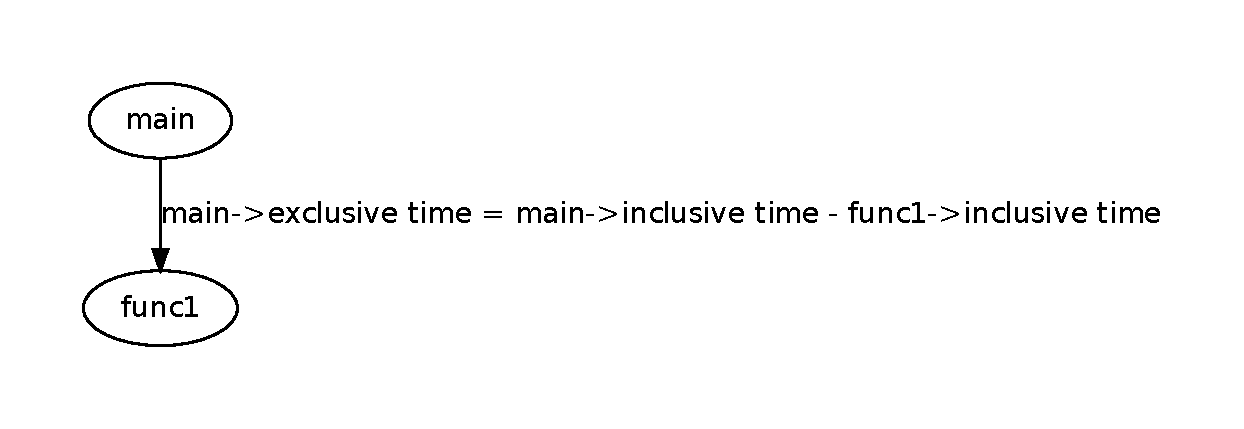
\includegraphics[scale=0.50]{Tree1}
	\captionof{figure}{Ajout d'un second noeud enfant}
\end{center}

L'opération est répétée jusqu'à la fin de l'analyse du fichier de traces.\\


L'un des objectifs du profiling est de pouvoir comparer les temps d'exécution de différentes instances d'une fonction. Nous avons avant tout besoin de détecter les fonctions redondantes du fichier d'entrée, puis les considérer comme des instances différentes d'une même fonction.
L'analyseur reparcourt donc les fonctions parsés, identifie celles ayant le même nom, puis les stocke dans une structure, en renseignant le nombre d'instances.\\
Les données recueillies sont ainsi sérialisées dans un fichier de sortie, puis interprétées en vue de produire un diagramme gnuplot 


Une autre fonctionnalité du profiler est de corréler les données statiques et dynamiques d'une fonction, à savoir confronter le temps d'exécution et le nombre de load/store. Dans cette optique, l'outil possède une grammaire lui permettant de reconnaître les données issues de l'instrumentation statique:

\begin{verbatim}
FUNCTION NAME RETLINE
NUMERIC LOAD RETLINE
NUMERIC MUL NUMERIC LOAD RETLINE
NUMERIC STORE RETLINE
NUMERIC MUL NUMERIC STORE RETLINE
\end{verbatim}

Une fois les données statiques consommées, on peut calculer le nombre de loads et de store par fonction, puis, en parcourant la liste des fonctions déjà stockées, faire correspondre le nombre de load/store aux données dynamiques précédemment analysées.\\

Enfin, l'outil propose également une corrélation entre les sorties statique et dynamique en analysant le fichier de traces statique. Cette corrélation nous fournit le nombre d'opérations load et store par fonction\\

Enfin, l'outil se propose de générer un graphe d'appel des fonctions, en procédant au parcours de l'arbre n-aire construit. Il produit en sortie un fichier compréhensible par l'outil dot. 

\begin{center}
	\includegraphics[scale=0.50]{/home/aurele/MIHP/CPA/Projet/myproof/Partie3/MyProfCallGraph}
	\captionof{figure}{Functions Call Graph}
\end{center}
\end{document}
